\documentclass[11pt,a4paper]{article}
\usepackage[utf8]{inputenc}
\usepackage[spanish]{babel}
\usepackage{amsmath}
\usepackage{amsfonts}
\usepackage{amssymb}
\usepackage{graphicx}
\usepackage[left=2cm,right=2cm,top=2cm,bottom=2cm]{geometry}
\author{Barrera Vazquez Omar}
\title{Universidad Politécnica de la Zona Metropolitana de Guadalajara}
\begin{document}

\maketitle

\begin{figure}[h]
\begin{center}

\includegraphics[scale=1]{1.jpeg}
\end{center}
\end{figure}

\begin{center}
\author{Sistemas Electrónicos de Interfaz\\
Barrera Vázquez Omar\\
Ing. Mecatrónica 4B\\}
\end{center}

\newpage

\section{Objetivo de la practica}

Reconocer el funcionamiento de las distintas configuraciones con las que trabaja un amplificador operacional, de tal manera que el alumno sepa identificar, calcular y configurar un amplificador en sus usos mas habituales como lo son: \emph{modo inversor, no inversor, restador, sumador, convertidor analogico-digital y digital- analogico}.

\section{Materiales}

En esta practica solo se hará uso de software por lo que se requiere de la previa instalación de los programas que se mencionan a continuación:

\begin{itemize}
\item Programa de diseño profesional de esquemas eléctricos \textbf{Orcad}
\item Programa de diseño de esquemas eléctricos \textbf{Proteus} en su version 8.0
\item Programa de diseño de esquemas eléctricos \textbf{Kicad} (este ultimo opcional a Orcad
\end{itemize}

\section{Desarrollo de la practica}

\subsection{Amplificador operacional en modo inversor}

Un amplificador operacional en modo inversor, básicamente realiza dos acciones con la tension que recibe y son las siguientes:

\begin{itemize}
\item un amplificador como su nombre lo dice, toma una señal eléctrica ya de en corriente AC o DC y la amplifica, esto por medio de una ganancia obtenida, ejemplo, si se tiene una señal senoidal de 5V pico, y el amplificador nos da una ganancia de 10, a la salida obtendremos un voltaje total de 50V, por lo que realmente el voltaje de entrada se multiplico por la ganancia,
\item otra acción que realiza  el amplificador operacional en modo inversor, es que la corriente nos la da contraria a la de entrada, ejemplo, si tenemos 5V de entrada, a la salida obtendremos un voltaje de -50V
\item la ganancia la obtenemos por la resistencia que se encuentra en lazo cerrado entre la resistencia de la entrada de alimentación, como lo muestra la ecuación 1:
\begin{equation}
\Delta=-1\frac{RF}{R1}
\end{equation}
\end{itemize}

Cambien se puede observar en la figura 1, en donde se muestra un amplificador inversor

\begin{figure}[ht]
\begin{center}
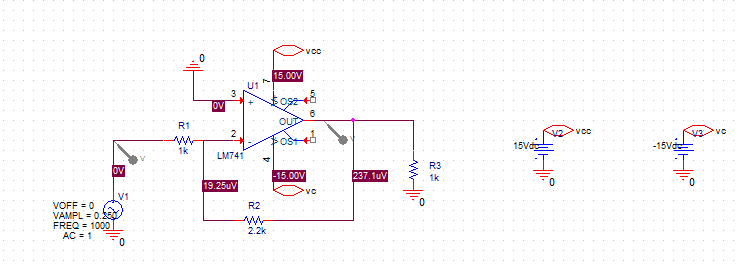
\includegraphics[scale=0.5]{1.PNG}
\caption{amplificador inversor esquema}
\end{center}
\end{figure}
\begin{figure}[h]
\begin{center}
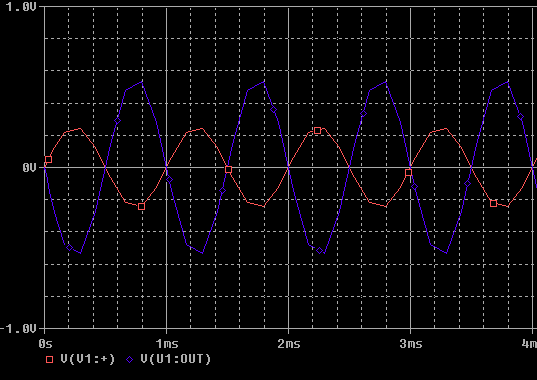
\includegraphics[scale=0.5]{2.PNG}
\caption{amplificador inversor esquema}
\end{center}
\end{figure}
\subsection{Amplificador no inversor}

Este amplificador no inversor, lo que realiza es casi exactamente lo mismo que el amplificador inversor, con la excepción de que este no da en contraria la señal de la corriente, unicamente termina por amplificarla, por lo que, nos entrega la misma señal multiplicada por la ganancia. Para obtener su ganancia es la siguiente que se observa en la formula 2:

\begin{equation}
\Delta=1\frac{RF}{R1}
\end{equation}

Para obtener su voltaje de salida, al igual que el inversor, se multiplica su voltaje de entrada por la ganancia, por lo que se obtiene la formula 3:

\begin{equation}
Vo=\Delta*Vin
\end{equation}

Se observa el circuito y la forma de onda en la figura 2(a y b):

\begin{figure}[ht]
\begin{center}
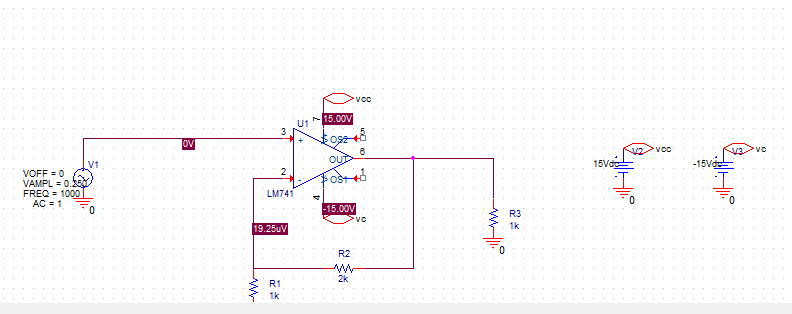
\includegraphics[scale=0.5]{3.PNG}
\caption{esquemático de amplificador no inversor}
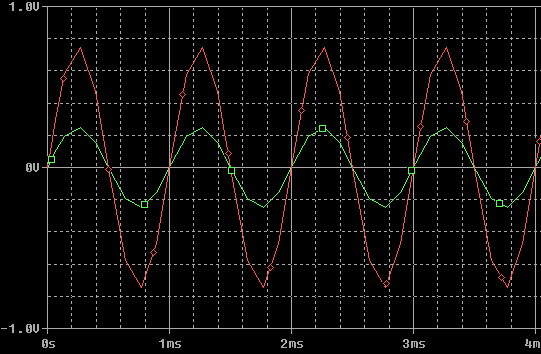
\includegraphics[scale=0.5]{4.PNG}
\caption{simulación en Orcad de Vin y Vout de no inversor}
\end{center}
\end{figure}

\subsection{Amplificador sumador}

Un amplificador sumador, toma los voltajes de entrada, tanto de positivo como el negativo, inmediatamente hace una suma algebraica de los voltajes, correspondiente entrega el voltaje que da el total de la suma de los voltajes. Este circuito es un tanto mas complejo de obtener, primeramente su ganancia se obtiene con la siguiente formula 4:

\begin{equation}
\Delta=\frac{RF}{R1}
\end{equation}

Para obtener su voltaje de salida se obtiene por medio de la formula 5:

\begin{equation}
Vo=-(V1*\frac{RF}{R1}+V2*\frac{RF}{R2}+V3*\frac{RF}{R3}
\end{equation}

En la siguientes imágenes 3 (a y B) se observa el diagrama de un amplificador sumador así como sus voltajes de entrada y salida correspondientes:

\begin{figure}[ht]
\begin{center}
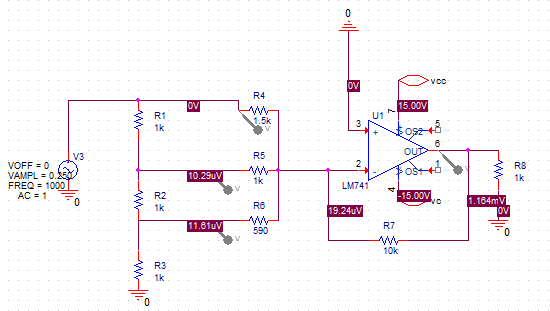
\includegraphics[scale=0.5]{5.PNG}
\caption{esquemático de amplificador sumador}
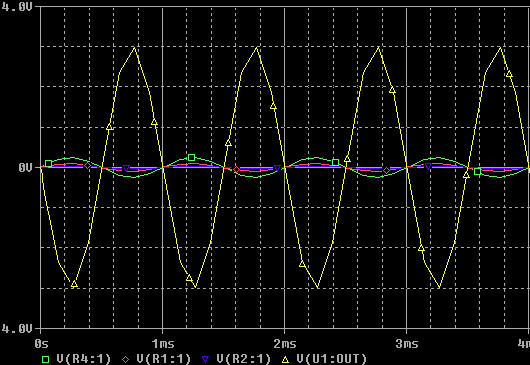
\includegraphics[scale=0.5]{6.PNG}
\caption{simulación de voltajes de entrada y salida de sumador}
\end{center}
\end{figure}

\subsection{Amplifico restador}

El amplificador restador tiene una manera parecida al sumador, con la excepción de que este toma como referencia los dos voltajes de entrada, tanto positivo como negativo, por lo que al voltaje positivo le resta lo que se encuentra en la entrada del voltaje negativo, para obtener el voltaje de salida del amplificador, utilizamos la formula 6:

\begin{equation}
Vo=[1+\frac{RF}{R1}]*[\frac{Rx}{R2+Rx}*V1-\frac{RF}{R1+RF}*100mV
\end{equation}

La figura 4 (a y b) nos muestran tanto el esquemático del amplificador operacional restador y su simulación de voltajes de entrada y salida respectivamente:

\begin{figure}[ht]
\begin{center}
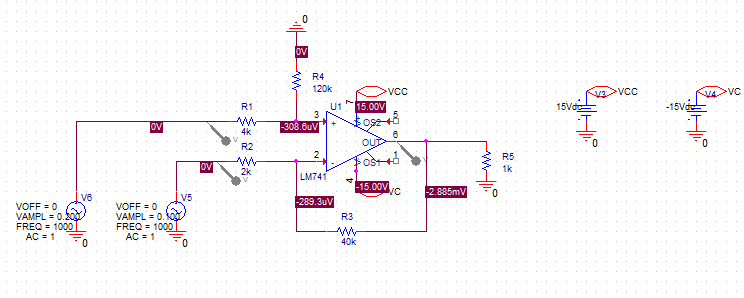
\includegraphics[scale=0.5]{7.PNG}
\caption{esquemático de amplificador restador}
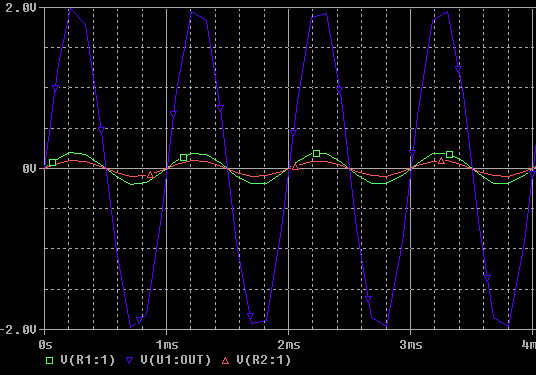
\includegraphics[scale=0.5]{8.PNG}
\caption{simulaciones de un amplificador restador}
\end{center}
\end{figure}


\subsection{Convertidor Digital-analogico}

El convertidor digital-analogico, es la utilización de amplificadores operacionales en modo sumador, el cual recibe una gran cantidad de entradas de voltajes por medio de sus voltajes de referencias, donde cada señal tendrá un voltaje distinto, por lo que, la suma de los voltajes, sera la señal analógica como lo muestra la figura 5:

\begin{figure}[ht]
\begin{center}
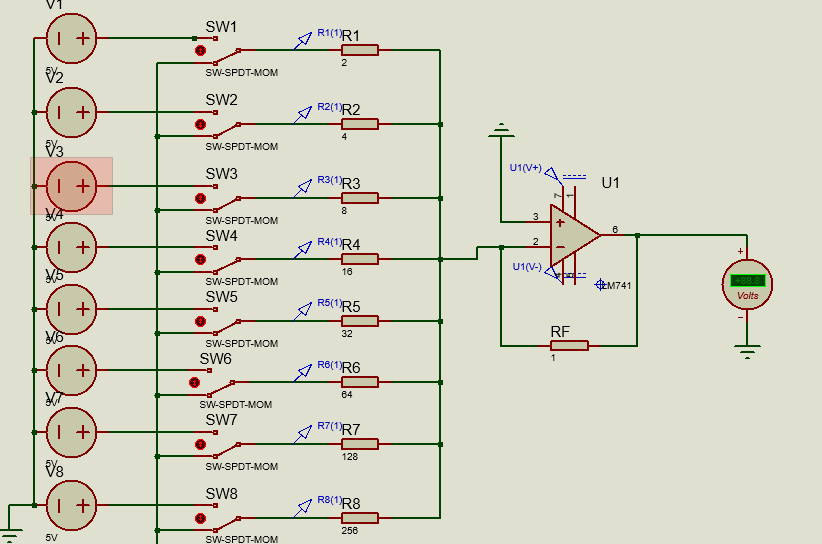
\includegraphics[scale=0.5]{10.PNG}
\caption{convertidor de digital-analogico}
\end{center}
\end{figure}


\subsection{Amplificador analogico-digital}

Este amplificador trabaja de manera inversa al convertidor digital analogico, toma una señal analógica y la compara con un voltaje de referencia el cual se convierte en el encendido de leds en modo binaria a la salida del amplificador, a este tipo de trabajo del amplificador se le llama modos comparador, porque básicamente compara el voltaje de la señal con un voltaje de regencia, un ejemplo lo podemos observar en la figura 6:

\begin{figure}[ht]
\begin{center}
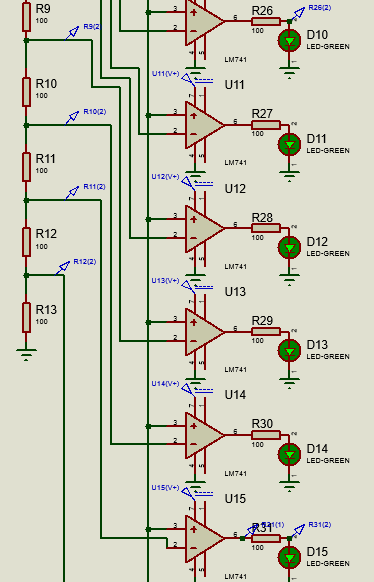
\includegraphics[scale=0.5]{9.PNG}
\caption{convertidor análogo-digital}
\end{center}
\end{figure}





\end{document}